\documentclass{article}

\usepackage{listings}
\usepackage{graphicx}

\title{How to make a Linux Distro (WIP)}

\renewcommand{\maketitle}{
	\begin{center}
		{\huge\bfseries
		How to make a Linux Distro (WIP)}
		\vspace{.25em}

		Funy Monkey --- Last Updated: DATE 
	\end{center}
}

\begin{document}

\maketitle
\tableofcontents

\section{Foreword}
	\textit{\textbf{Why would you want to make your own Linux Distro?}}

	When needing to deploy multiple Systems it can sometimes be easier to just run the installer of your own Linux Distro and be done with it, instead of having to either do it Manually or use a Script. It can also be very fun!
	\\And it can help you learn the inner workings of a Linux Distro.

	\textit{\textbf{i gotta add more shit here!}}

\section{From Scratch}
\label{Scratch}
\textbf{NOT RECOMMENDED!}
\subsection{The Base}
	\label{ScratchBase}
	Depending on how minimal you want your Distro to be, it is \textbf{Very reccommended} that you follow the \ahref{https://linuxfromscratch.org/lfs}{Linux from Scratch Book}

	The \ahref{https://linuxfromscratch.org/lfs}{Linux from Scratch Book} is already \textbf{Very, Very} Minimal, so we will be going through the \textbf{ABSOLUTE MINIMUM} for a \textit{working} Linux System 
		\subsubsection{Workspace}
			Create a Folder for the Workspace and make all needed Folders
			
			\begin{lstlisting}
	mkdir -v <WorkspaceDirectory>
	cd <WorkspaceDirectory>
	mkdir -v rootfs
			\end{lstlisting}

			It can be very helpful to use a tool like \ahref{https://git-scm.com}{git} to easily revert changes
		\subsubsection{Linux Kernel}

			Download and Extract the Linux Kernel (There probably will be newer kernels than the one on the link shown here. If you want a newer Linux Kernel go to \ahref{https://www.kernel.org}{The linux kernel Website} and download it from there.)
			\begin{lstlisting}
	wget https://cdn.kernel.org/pub/linux/kernel/v5.x/linux-5.12.8.tar.xz
	tar -xvf linux-5.12.8.tar.xz
	cd linux-5.12.8
			\end{lstlisting}
			Now we need to \textbf{Compile and Configure} the Kernel, depending on what this must run on this can be either very Simple or Complex and Time Consuming.
			\begin{lstlisting}
	make mrproper
	make defconfig
	make menuconfig
			\end{lstlisting}
			For documentation on comfiguring the Linux Kernel, check out \ahref{https://linuxfromscratch.org/lfs/view/stable/chapter10/kernel.html}{This} Segment of the Linux From Scratch Book and the \ahref{https://wiki.gentoo.org/wiki/Kernel/Configuration}{Gentoo wiki Page} on Configuring the Kernel
			\begin{lstlisting}
	make -j<threads to be used> # use the command "nproc --all" to find out how many Threads are on your System
	cp -iv arch/x86/boot/bzImage ../vmlinuz
	cd ..
			\end{lstlisting}
			Replace ``x86'' with another Architecture if you are not compiling the x86 Linux Kernel
		\subsubsection{Root Filesystem}
			The first File we need is the init which will initialize the System, it needs to be an Executable program.
			\begin{lstlisting}
	# Edit init.c with your favorite Text Editor #
	
	#include <stdio.h>
	#include <unistd.d>

	int main() {
		printf("Hello, Linux World!\n");
		sleep(0xFFFFFFFF);
		return 0;
	}

	# Edit init.c with your favorite Text Editor #
	gcc -static init.c -o rootfs/init
			\end{lstlisting}
			\subsubsection{Booting}
			\begin{lstlisting}
	(cd rootfs && find . | cpio -o -H newc | gzip > ../rootfs.cpio.gz)
	qemu-system-x86_64 <other qemu parameters (for example: -m 128M)> -kernel vmlinuz -initrd rootfs.cpio.gz
			\end{lstlisting}
			When booted, it should print out ``Hello, Linux World!'' as shown here.
			\\
			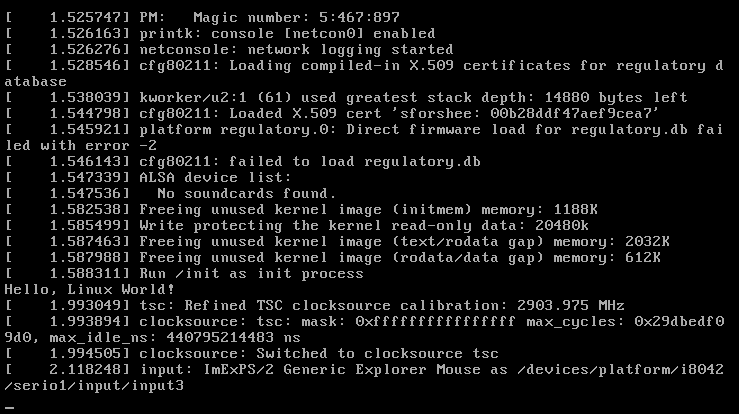
\includegraphics{hellolinuxworld}
		
		\subsection{Adding Programs}
		Now we have a \textit{working} Linux System, albeit very useless.
		So lets add a shell, in this case we will use \ahref{https://www.gnu.org/software/bash}{Bash}.
		\subsubsection{Bash}
		\label{ScratchAddBash}
		\paragraph{Dynamic Linking}
		To dynamically compile Bash, the Linux System will need all of Bash's Dependencies, which are
		\begin{enumerate}
			\item glibc
			\item ncurses
			\item readline
		\end{enumerate}
		And you will of course need the Dependencies of those Programs as well.
		\\
		You could also follow the \ahref{https://linuxfromscratch.org/lfs/view/stable/chapter05/binutils-pass1.html}{Linux from Scratch Book Compilation Segment} up until Bash.

		Now, to Download and Compile Bash:
		\\
		Remember that there might be a newer Version of Bash on the \ahref{https://www.gnu.org/software/bash}{Bash Website}
		\begin{lstlisting}
	wget https://ftp.gnu.org/gnu/bash/bash-5.1.tar.gz
	tar -xf bash-5.1.tar.gz
	cd bash-5.1
	./configure --prefix=/usr		    \
		    --build=$(support/config.guess) \
		    --host=x86_64		    \
		    --without-bash-malloc
	make
	make DESTDIR=<WorkspaceDirectory>/rootfs install
	cd ..
		\end{lstlisting}
		Replace ``x86_64'' with another Architecture if you are not compiling for x86_64

		Bash will now reside in /usr/bin/bash, but it should be moved to /bin/bash
		\begin{lstlisting}
	cd rootfs
	mkdir -v bin
	mv usr/bin/bash bin/bash
		\end{lstlisting}
		\paragraph{Static Linking}
		Static Compilation does not need any of Bash's dependencies to be in the System, instead it is just one Singular File.

		\ahref{https://www.musl-libc.org}{musl} is needed for true Static linking
		\\ Either install it with a Package Manager of choice or build it from Source.

		Set ``musl-gcc'' as the C Compiler and set CFLAGS.
		\begin{lstlisting}
	export CC="musl-gcc"
	export CFLAGS="-static"
		\end{lstlisting}
		Now, to Download and Compile Bash:
		\\
		Remember that there might be a newer Version of Bash on the \ahref{https://www.gnu.org/software/bash}{Bash Website}
		\begin{lstlisting}
	wget https://ftp.gnu.org/gnu/bash/bash-5.1.tar.gz
	tar -xf bash-5.1.tar.gz
	cd bash-5.1
	CFLAGS="$CFLAGS -Os" ./configure --prefix=/usr			 \
					 --build=$(support/config.guess) \
					 --host=x86_64			 \
					 --without-bash-malloc
	make
	make DESTDIR=<WorkspaceDirectory>/rootfs install
	cd ..
		\end{lstlisting}
		Replace ``x86_64'' with another Architecture if you are not compiling for x86_64

		Bash will now reside in /usr/bin/bash, but it should be moved to /bin/bash
		\begin{lstlisting}
	cd rootfs
	mkdir -v bin
	mv usr/bin/bash bin/bash
		\end{lstlisting}
		\subsubsection{BusyBox}
			\paragraph{Dynamic Linking}
			\paragraph{Static Linking}	
		\subsubsection{Package Manager}	
			\paragraph{The Packages}
			\paragraph{The Manager}
		\subsection{The Boot Loader}
		\subsection{Making an Installer}
\section{Arch Based}
\textbf{You can either generate an Arch Linux ISO with \ref{Archiso} Archiso or \ref{ArchIsoEdit} edit an ISO from the \ahref{https://archlinux.org/download}{Arch Linux Website}}
\subsection{Archiso}
	\label{Archiso}
	\textbf{YOU NEED TO BE ON AN ARCH LINUX SYSTEM!}

	First install Archiso:
	\begin{lstlisting}
	sudo pacman -S archiso
	\end{lstlisting}
	Archiso comes with 2 profiles, \textbf{releng} and \textbf{baseline}.
	\\
	Copy the Profile of your Choice to a Directory of your Choice, where <profile> is either \textbf{releng} or \textbf{baseline}:
	\begin{lstlisting}
	cp -r /usr/share/archiso/configs/<profile> <directory>
	\end{lstlisting}

\subsection{ISO Editing}
	\label{ArchIsoEdit}
\section{Debian Based}
\section{Ubuntu Based}
\section{Generic}
\section{Branding}
\section{Afterword}
\section{Sources}
\ref{Scratch} \ahref{https://www.linuxfromscratch.org/lfs}{Linux From Scratch Book}

\ref{ScratchBase} \ahref{https://stackoverflow.com/a/30056182}{Stackoverflow Answer} 

\ref{ScratchAddBash} \textit{\textbf{Dynamic:}}
\ahref{https://linuxfromscratch.org/lfs/view/stable/chapter06/bash.html}{Linux From Scratch Bash Page}
\textit{\textbf{Static:}} \ahref{https://github.com/robxu9/bash-static/blob/master/build.sh}{Static Bash Build Script}

\ref{Archiso} \ahref{https://wiki.archlinux.org/title/archiso}{Archiso Arch Wiki Page}
\end{document}
